\documentclass[a4paper,10pt]{article}
\usepackage[utf8]{inputenc}
\usepackage[margin=22mm]{geometry}
\usepackage{amsmath,amssymb,graphicx,booktabs,array,tabularx}
\usepackage[hidelinks]{hyperref}
\usepackage{caption}
\renewcommand{\thesection}{S\arabic{section}}
\renewcommand{\thetable}{S\arabic{table}}
\renewcommand{\thefigure}{S\arabic{figure}}
\numberwithin{equation}{section}
\setlength{\parskip}{4pt}
\setlength{\parindent}{0pt}
\setlength{\emergencystretch}{2em}
\graphicspath{{figures/validation/}}
\title{\textbf{Supplementary Material}\\[3pt]
Numerical verification of multilayer tracer transport}
\author{Companion to the multilayer platelet--fibrin study}
\date{12 October 2026}
\begin{document}
\maketitle
\section{Scope, geometry, and implementation}
This supplement distinguishes implementation checks, analytical first-passage benchmarks, and discretization sensitivity. These questions are not equivalent to biological validation \cite{Slater2021}. Sections S1--S7 preserve the historical fixed-mask and local continuous-geometry experiments with whole-proposal rejection. Section S8 documents the subsequent full-common-domain reflection protocol, including cohesive solids, used for the homogeneous pilot in the main text. No simulation was rerun to compile this supplement.

The historical phase is closed provisionally, with an unresolved long-horizon escape-equivalence interval. Its conclusions remain conditional on the tested geometry and boundary rule and are not pooled with, or transferred automatically to, the current main-text cohort.

\subsection*{Two different geometric settings}
The fixed-mask temporal study uses 50 layers of thickness $H=70$ nm, total thickness $L=3.50~\mu$m, and a $47.6\times47.6~\mu$m field rasterized as $50\times256\times256$ cells. Its accessible-center mask is based on anisotropic EDT distances between raster sites.

The subsequent geometry and transport studies use a central $5.95\times5.95\times5.00~\mu$m region of the same saved 50-layer mechanical realization (base seed 4000, $f_0=2.2$ nN, mechanical time 10 s). Here $H=100$ nm is the assumed physical slab thickness, whereas $h_z=H/m$ is a numerical subdivision. The reference therefore contains 50 mechanical layers even when it contains 1600 numerical cells in $z$.

Each backbone segment is represented by a planar capsule, and each platelet by a planar disk, extruded across its own slab. Cohesive links are not added as new solid primitives in this geometry audit. This is a continuous interpretation of a layered model, not a reconstructed curved 3D fiber network or a set of spherical platelets. A halo of neighboring obstacles is retained for clearance queries; 2186 primitives enter the local detector.

The two size scenarios use $(a,D)=(0.10~\mu\mathrm{m},1.0~\mu\mathrm{m}^2/\mathrm{s})$ and $(0.25~\mu\mathrm{m},0.4~\mu\mathrm{m}^2/\mathrm{s})$. They change both steric size and diffusion. The final two refinements concern only the larger tracer.

\subsection*{Tracer update and boundary ordering}
All tracers are noninteracting and released inside the domain, not injected through $z=0$. Independent Gaussian coordinates generate each free proposal,
\begin{equation}
\mathbf R^*=\mathbf R+\sqrt{2D\Delta t}\,\boldsymbol{\eta},
\qquad \boldsymbol{\eta}\sim\mathcal N(\mathbf 0,I_3).
\end{equation}
The entire straight proposal is checked up to its first external boundary. A voxel supercover visits every touched cell, including edge/corner contacts. The continuous detector instead checks swept-sphere clearance against the extruded solid. A solid or lateral contact before, or tied with, an axial exit causes whole-proposal rejection and consumes the step. Otherwise the first free $z$ crossing absorbs the tracer. Escape time is recorded at the step endpoint, not as an exact Brownian first-contact time.

In the local test, $z=0$ and $z=5~\mu$m are absorbing for the tracer center, while the artificial ROI sides reject crossing proposals. Those sides can remove paths that would exist in the complete clot. Network mechanics remains frozen throughout the 100 s transport clock.

\subsection*{Implementation checks}
Checks include 16 transport-kernel tests of segment traversal, anisotropic cells, edges/corners, face ordering, obstacles before exit, final-step duration, and censoring. Independent continuous checks include 1200 segment-distance minimizations, analytic tangency cases, 4096 point-clearance comparisons, and 20000 detector comparisons before each recent refinement. The continuous distance search uses a bounding-volume hierarchy and conservative clearance bounds; it does not infer safety solely from free endpoints. These tests verify specified rules, not exact reflected Brownian motion.

\section{Estimands, uncertainty, and equivalence}
Let $T_i$ be first exit through either axial face and let $T_c$ be the common observation horizon. With administrative right censoring,
\begin{align}
\widehat P_{\rm esc}(t)&=N^{-1}\sum_i\mathbf 1(T_i\le t),\\
\widehat S(t)&=1-\widehat P_{\rm esc}(t),\\
\widehat{\mathrm{RMST}}(T_c)&=N^{-1}\sum_i\min(T_i,T_c)
=\int_0^{T_c}\widehat S(t)\,dt .
\end{align}
Every censored history contributes $T_c$. The mean is not conditioned on escape, and positive $S(T_c)$ does not establish permanent capture \cite{Redner2001,RoystonParmar2013}. Exact integration of each empirical step-survival curve was checked against its reported RMST.

All differences are the coarser method minus the finer reference. Working margins were fixed at $\pm2$ percentage points (pp) for escape probability and $\pm3\%$ for relative RMST. Equivalence requires the complete 95\% confidence interval to fall inside the margin. A crossing interval is inconclusive; an interval entirely beyond a margin is outside. Joint equivalence requires \emph{both} indicators to pass at the specified horizon.

These tolerances are exploratory numerical choices, not universal physiological thresholds. A small point estimate or a nonsignificant difference from zero is insufficient to establish equivalence \cite{Lakens2017}. The 95\% containment rule is more stringent than the 90\% interval convention used for standard TOST at the 5\% level; it is not presented here as that standard TOST procedure.

\subsection*{Sampling units}
The $H=70$ nm study uses paired differences of 16 batch means (1000 tracers per batch), with Student intervals on 15 degrees of freedom. Its seeds and starting sites are paired, but increments are not coupled step by step across resolutions.

The $H=100$ nm precision and nested-refinement studies use 8192 individually paired histories (32 batches of 256) on one fixed geometry. For a paired observable $Y$, the interval is
\begin{equation}
\overline{\Delta Y}\ \pm\ t_{0.975,N-1}
\frac{s_{\Delta Y}}{\sqrt N}.
\end{equation}
Relative RMST divides this interval by the observed mean of the finer method. A delta-method sensitivity includes uncertainty of that denominator; it changes none of the decisions in the final refinement. These intervals characterize tracer Monte Carlo uncertainty, not between-clot or between-mechanical-seed variability.

Wilson intervals describe pointwise survival. At zero observed discordance, a conservative exact bound avoids assigning zero uncertainty to an escape difference. Pointwise bands do not provide simultaneous coverage of the entire survival curve. Multiple horizons share histories; successive refinement stages are exploratory rather than a familywise-controlled sequence.

\subsection*{Reuse without double counting}
The original local pilot had 512 histories per size and method. The later precision study used 8192 new initial centers per size; its new-only analysis is primary, and pooled pilot-plus-new results are separate sensitivity analyses. The 0.03125 and 0.015625 ms stages each reuse those same 8192 centers and earlier histories. They add methods, not independent mechanical replicates or additional pairs to the primary sample.

\clearpage
\section{Fixed-mask temporal verification at H = 70 nm}
The primary comparison is $\Delta t=0.125$ versus $0.0625$ ms at $T_c=10,20,50,100$ s, for both tracer radii. Each radius and step uses 16000 trajectories, giving 64000 histories in total. Initial accessible voxel centers lie in the axial band $0.4L\le z<0.6L$ and a central in-plane disk. The same $50\times256\times256$ EDT mask is held fixed.

\begin{table}[!htbp]
\centering\small
\setlength{\tabcolsep}{4pt}
\caption{Fixed-mask temporal comparison: 0.125 minus 0.0625 ms. Both escape and RMST meet the working margins for all listed conditions. Intervals are paired 95\% confidence intervals across 16 Monte Carlo batches.}\label{tab:h70}
\begin{tabular}{@{}cccc@{}}
\toprule
$d$ ($\mu$m) & $T_c$ (s) & $\Delta P$ [CI] (pp) & $\Delta\mathrm{RMST}$ [CI] (\%) \\ \midrule
0.20 & 10 & $-0.281\ [-0.917,0.355]$ & $0.278\ [-0.763,1.320]$ \\
0.20 & 20 & $-0.031\ [-0.344,0.281]$ & $0.495\ [-0.863,1.852]$ \\
0.20 & 50 & $-0.006\ [-0.030,0.017]$ & $0.497\ [-0.938,1.931]$ \\
0.20 & 100 & $0.000\ [-0.031,0.031]$ & $0.496\ [-0.946,1.939]$ \\
0.50 & 10 & $-0.100\ [-0.951,0.751]$ & $0.246\ [-0.240,0.733]$ \\
0.50 & 20 & $-0.531\ [-1.504,0.441]$ & $0.477\ [-0.178,1.132]$ \\
0.50 & 50 & $-0.906\ [-1.771,-0.041]$ & $1.264\ [0.360,2.168]$ \\
0.50 & 100 & $-0.169\ [-0.713,0.376]$ & $1.618\ [0.323,2.913]$ \\
\bottomrule
\end{tabular}
\end{table}

All listed paired intervals meet the selected margins. The tightest case is the large-tracer RMST at 100 s: $1.618\%$ with interval $[0.323,2.913]\%$. At the fine step, the small tracer has no censored histories at 100 s, while the large tracer retains 1324/16000 histories, with RMST $35.5467$ s. Of the large-tracer starts, 198/16000 lie in components connected to neither axial face; none of those escaped.

The combined sample was fixed before completing its extension, guided by a pilot. A sensitivity analysis restricted to additional batches leaves some large-tracer comparisons inconclusive. It is not an independent confirmation of all the combined-sample decisions.

\begin{figure}[!htbp]
\centering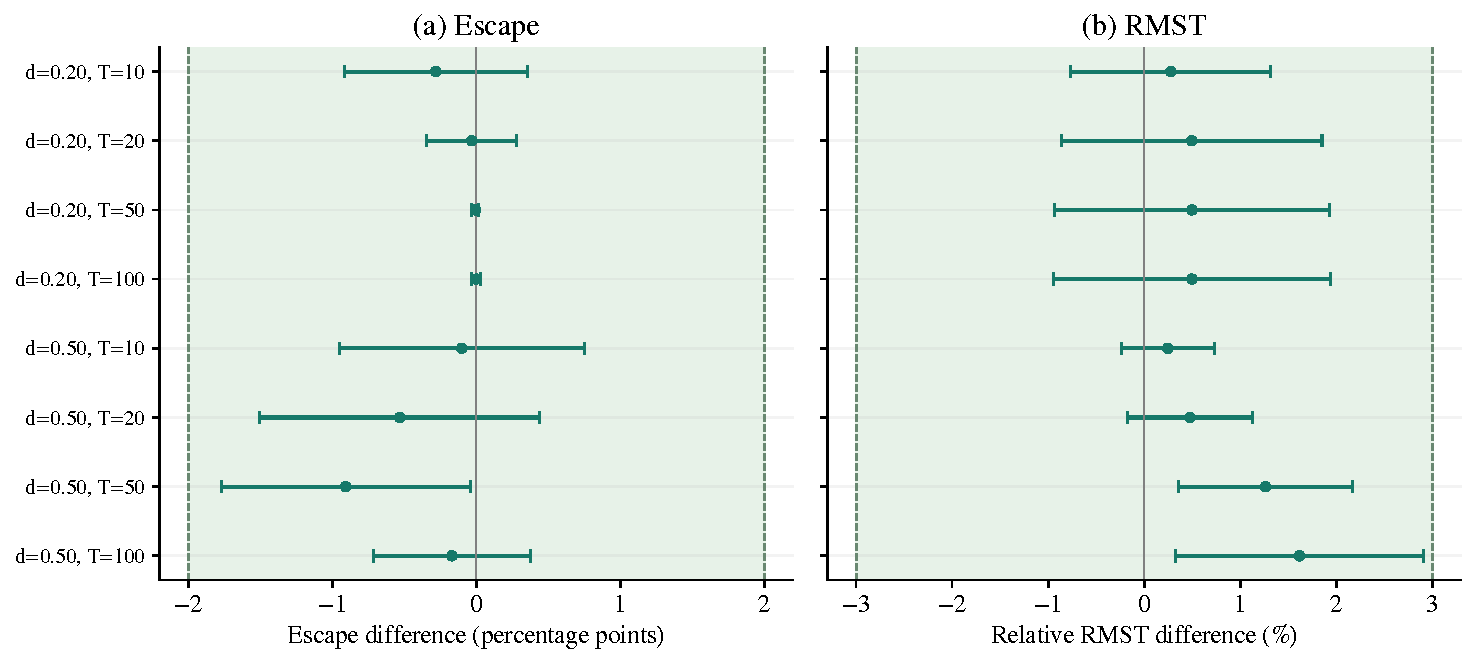
\includegraphics[width=\textwidth]{s1_h70_equivalence.pdf}
\caption{Fixed-mask temporal equivalence. Labels give diameter $d$ in $\mu$m and horizon $T$ in seconds. Bars are paired 95\% intervals across batches; shaded regions are the working margins.}
\end{figure}

This result supports a finite-step comparison on the specified EDT mask. It does not validate the 1 ms endpoint pilot, exact sphere--surface clearance, the $H=100$ nm geometry, other mechanical realizations, or moving obstacles. A five-step exploratory sweep at 10 s showed larger-step sensitivity; its 4000 histories per condition are not added again to the 16000-history primary cohort.

\clearpage
\section{Analytical control geometries}
The backward equation $D u''=-1$ provides mean-exit references in separable domains \cite{Redner2001}. For an interval with absorbing endpoints,
\begin{equation}
u(z)=\frac{z(L-z)}{2D}.
\end{equation}
For a reflecting wall at accessible coordinate $a$ and an absorbing endpoint $L$, with $\ell=L-a$,
\begin{equation}
u(z)=\frac{\ell^2-(z-a)^2}{2D},\qquad u'(a)=0,\quad u(L)=0.
\end{equation}
A straight channel with ideal reflecting lateral walls has the same axial first-passage law as the free interval. Whole-proposal rejection can instead suppress an axial displacement when its transverse part touches a wall, producing finite-step delay.

The absorbing-interval survival expansion is
\begin{equation}
S(t\mid z)=\frac4\pi\sum_{j=0}^\infty
\frac{\sin[(2j+1)\pi z/L]}{2j+1}
\exp\!\left[-D\left(\frac{(2j+1)\pi}{L}\right)^2t\right].
\end{equation}
For the mixed reflecting/absorbing case, with $x=z-a$ and $q_j=(j+1/2)\pi/\ell$,
\begin{equation}
S(t\mid x)=\sum_{j=0}^\infty
\frac{2(-1)^j}{\ell q_j}\cos(q_jx)e^{-Dq_j^2t}.
\end{equation}
The references are averaged over the actual sampled starting positions and integrated to the same $T_c$ as the simulation. They do not use the numerical collision detector. For the voxel controls, 512 and 1024 modes agreed in RMST to better than $10^{-8}$ s.

\subsection*{Voxel controls}
The free and wall controls have broad lateral domains. The wall occupies $z\le1.05~\mu$m; the straight channel has a $2\times2~\mu$m accessible cross-section. These domains prescribe \emph{center} accessibility directly and are not eroded by a tracer radius a second time. There are $3\times3\times8000=72000$ histories.

\begin{table}[!htbp]
\centering\small
\setlength{\tabcolsep}{4pt}
\caption{Voxel control geometries ($L=3.5~\mu$m, $D=1~\mu$m$^2$/s, $T_c=20$ s): 8000 trajectories per condition. Error is relative to the analytical RMST for the sampled initial positions.}\label{tab:obstacles}
\begin{tabular}{@{}lccccl@{}}
\toprule
Control & $\Delta t$ (ms) & RMST (s) & Analytical (s) & Error [CI] (\%) & Decision \\ \midrule
free & 1.0000 & 1.5695 & 1.5109 & $3.88\ [2.03,5.72]$ & Inconclusive \\
free & 0.1250 & 1.5137 & 1.5109 & $0.19\ [-1.62,1.99]$ & Within \\
free & 0.0625 & 1.5239 & 1.5109 & $0.86\ [-1.01,2.73]$ & Within \\
Planar wall & 1.0000 & 2.8294 & 2.7356 & $3.43\ [1.39,5.46]$ & Inconclusive \\
Planar wall & 0.1250 & 2.7772 & 2.7356 & $1.52\ [-0.47,3.52]$ & Inconclusive \\
Planar wall & 0.0625 & 2.7859 & 2.7356 & $1.84\ [-0.17,3.84]$ & Inconclusive \\
Straight channel & 1.0000 & 1.6395 & 1.5109 & $8.51\ [6.58,10.44]$ & Outside \\
Straight channel & 0.1250 & 1.5619 & 1.5109 & $3.37\ [1.45,5.29]$ & Inconclusive \\
Straight channel & 0.0625 & 1.5242 & 1.5109 & $0.88\ [-0.96,2.71]$ & Within \\
\bottomrule
\end{tabular}
\end{table}

The straight channel identifies a clear discrepancy at 1 ms: $8.51\%$ RMST error, outside the $\pm3\%$ tolerance. At 0.0625 ms, the free and channel means meet the margin, while the wall remains inconclusive. No impossible lower-face escapes occur in the wall case. Small observed survival-curve discrepancies do not establish a uniform 2 pp error bound.

\clearpage
\subsection*{Continuous-detector controls}
These controls use $L=5~\mu$m, uniform initial $z\in[2,3]~\mu$m and $D=1~\mu$m$^2$/s. A solid wall at $z\le1.5~\mu$m with tracer radius $0.1~\mu$m puts its accessible boundary at $a=1.6~\mu$m. The channel half-width is $1~\mu$m. Each case has 8192 trajectories at each of two steps.

\begin{table}[!htbp]
\centering\small
\setlength{\tabcolsep}{4pt}
\caption{Continuous-detector controls: $L=5~\mu$m, $D=1~\mu$m$^2$/s, $T_c=100$ s, and 8192 trajectories per condition. No control was repeated at the two later refined steps.}\label{tab:continuous-controls}
\begin{tabular}{@{}lcccc@{}}
\toprule
Control & $\Delta t$ (ms) & RMST (s) & Analytical (s) & Error [CI] (\%) \\ \midrule
free & 0.125 & 3.0651 & 3.0840 & $-0.61\ [-2.40,1.17]$ \\
free & 0.0625 & 3.0557 & 3.0840 & $-0.92\ [-2.69,0.86]$ \\
wall & 0.125 & 5.4037 & 5.3336 & $1.31\ [-0.65,3.28]$ \\
wall & 0.0625 & 5.4004 & 5.3336 & $1.25\ [-0.72,3.22]$ \\
channel & 0.125 & 3.1090 & 3.0840 & $0.81\ [-1.01,2.63]$ \\
channel & 0.0625 & 3.0655 & 3.0840 & $-0.60\ [-2.40,1.20]$ \\
\bottomrule
\end{tabular}
\end{table}

\begin{figure}[!htbp]
\centering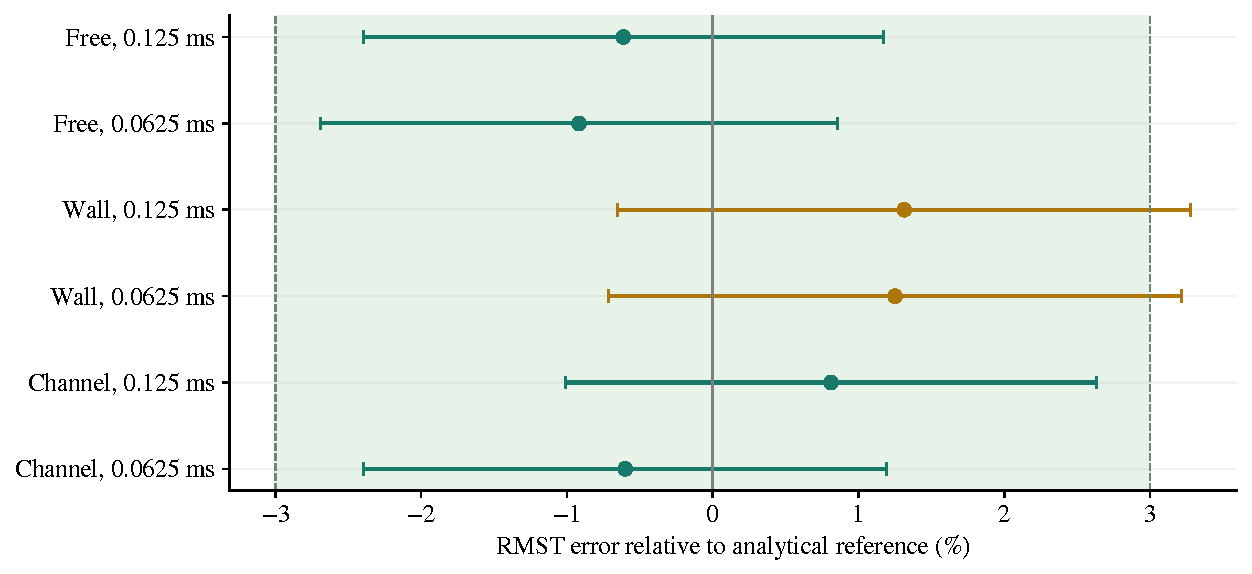
\includegraphics[width=.92\textwidth]{s3_continuous_controls.pdf}
\caption{Continuous-detector RMST errors and 95\% intervals relative to the analytical controls. Green intervals meet the 3\% margin; amber intervals are inconclusive.}
\end{figure}
The wall upper interval remains $3.22\%$ at 0.0625 ms. All six conservative uniform survival-error bounds exceed 2 pp, despite observed maxima of roughly 0.8--1.2 pp. Thus analytical verification is informative but not globally closed. No full-control suite was rerun at 0.03125 or 0.015625 ms; later steps retain the same detector and boundary rule.

\clearpage
\section{Spatial geometry and transport comparison}
For a cell $C$ and solid set $\mathcal S$, the conservative admission rule is
\begin{equation}
\min_{\mathbf x\in C,\mathbf y\in\mathcal S}
\|\mathbf x-\mathbf y\|\ge a+10^{-12}~\mu\mathrm{m}.
\end{equation}
A partially invalid cell is excluded completely. Refinement can recover valid parts without changing the underlying solid. The tested resolutions have $h_{xy}=11.621$ or $5.811$ nm and $h_z=6.25$ or $3.125$ nm; all span the same local ROI and 50 physical layers.

\begin{table}[!htbp]
\centering\small
\setlength{\tabcolsep}{4pt}
\caption{Local safe-cell geometry. Accessible volume is normalized by the entire region of interest (ROI); through-connected volume is normalized by accessible volume. Exclusion is normalized by valid points in the fresh continuous-reference sample.}\label{tab:geometry}
\begin{tabular}{@{}ccccccc@{}}
\toprule
$d$ ($\mu$m) & $h_{xy}$ (nm) & $h_z$ (nm) & Accessible (\%) & Components & Through (\%) & Excluded (\%) \\ \midrule
0.20 & 11.621 & 6.250 & 53.782 & 120 & 99.995 & 3.312 \\
0.50 & 11.621 & 6.250 & 18.328 & 315 & 97.814 & 5.664 \\
0.20 & 11.621 & 3.125 & 54.304 & 152 & 99.995 & 2.364 \\
0.50 & 11.621 & 3.125 & 18.583 & 332 & 97.767 & 4.365 \\
0.20 & 5.811 & 6.250 & 54.203 & 299 & 99.995 & 2.555 \\
0.50 & 5.811 & 6.250 & 18.618 & 470 & 97.789 & 4.257 \\
0.20 & 5.811 & 3.125 & 54.721 & 296 & 99.995 & 1.634 \\
0.50 & 5.811 & 3.125 & 18.873 & 574 & 97.754 & 2.936 \\
\bottomrule
\end{tabular}
\end{table}

Six-face adjacency defines connectivity; edge/corner-only contacts do not connect components. A main component occupies at least 1\% of accessible volume. A through component touches both external $z$ faces. No $z$-face contact does not imply a completely enclosed physical cavity, because the ROI has artificial sides.

The final per-axis comparisons require: relative accessible-volume change below 3\%; unchanged identities/counts of main and main-through components; unchanged presence of a through path; through-volume-fraction change below 3 pp; and no observed invalid admissions. All four final diameter-by-axis comparisons meet these criteria. Main-component identities were checked with physically matched points, not counts alone. Total small-component counts still change.

\begin{figure}[!htbp]
\centering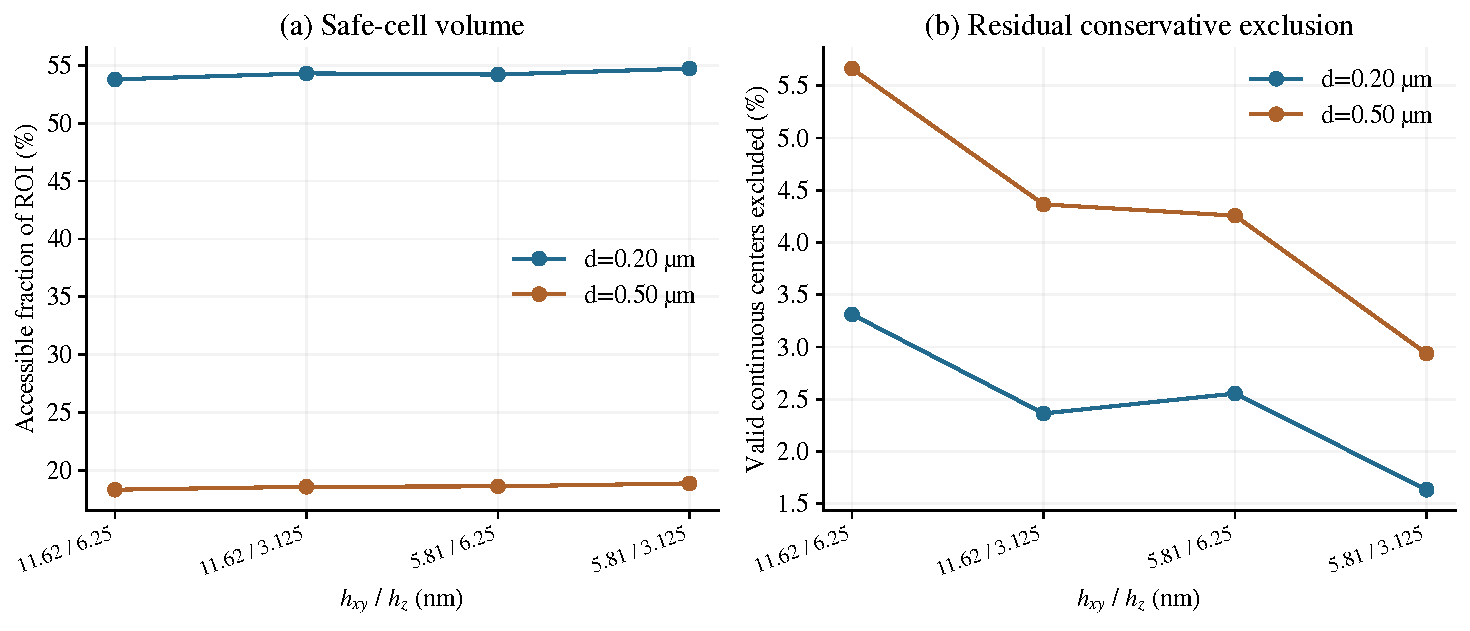
\includegraphics[width=\textwidth]{s2_spatial_geometry.pdf}
\caption{Safe-cell volume and residual exclusion relative to a fresh continuous-reference sample of 200000 points. The cell volumes are exact raster counts; the exclusion estimates carry sampling uncertainty. The two axes have different denominators.}
\end{figure}

\clearpage
\subsection*{Residual error and kinetic comparison}
The finest safe-cell mask retains 54.7214\% of ROI volume for diameter $0.20~\mu$m and 18.8731\% for $0.50~\mu$m. The continuous-reference estimates are 55.5840\% and 19.4285\%, respectively. Among valid continuous-reference points, the fine grid excludes 1.634\% (95\% Wilson CI $[1.562,1.711]\%$) and 2.936\% ($[2.773,3.109]\%$). This is not the same denominator or criterion as a 3\% change between grids.

Checks included 76 block-labeling comparisons against full-volume labeling, conservation of parent safe cells under subdivision, 16384 direct cell--solid distance comparisons, and zero observed false admissions in 220000 reference positions per configuration and radius. These are finite checks under the idealized geometry, not anatomical error bounds.

A subsequent precision study compared transport on the finest safe-cell mask with the continuous detector at the same 0.125 ms step, and compared two continuous steps. It used 8192 new paired starts per diameter, conditioned to be valid in all three initial comparison masks.

\begin{table}[!htbp]
\centering\small
\setlength{\tabcolsep}{4pt}
\caption{Precision study at 100 s: 8192 paired trajectories per diameter and method. Cells denote the finest safe-cell mask at 0.125 ms; continuous geometry uses the same solid. None of these four comparisons establishes joint equivalence.}\label{tab:bridge}
\begin{tabular}{@{}clcc@{}}
\toprule
$d$ & Comparison (ms) & $\Delta P$ [CI] (pp) & $\Delta$RMST [CI] (\%) \\ \midrule
0.20 & Cells -- continuous & $-0.01\ [-0.04,0.01]$ & $3.97\ [1.57,6.36]$ \\
0.20 & 0.125 -- 0.0625 & $0.00\ [-0.04,0.04]$ & $0.62\ [-1.80,3.04]$ \\
0.50 & Cells -- continuous & $-1.29\ [-2.67,0.08]$ & $1.52\ [0.35,2.69]$ \\
0.50 & 0.125 -- 0.0625 & $-2.17\ [-3.57,-0.78]$ & $2.02\ [0.81,3.23]$ \\
\bottomrule
\end{tabular}
\end{table}

For the small tracer, the cell-versus-continuous RMST difference remains $3.97\%$ with a $[1.57,6.36]\%$ interval. For the large tracer, RMST meets the margin but escape remains inconclusive. The small-tracer temporal upper RMST limit is $3.037\%$, just above 3\%; it is not rounded into a pass.

Consequently, stability of local geometric metrics is not closure of spatial transport convergence. The voxel and continuous methods must not be described as interchangeable. The finest full-domain grid would require more than $10^{11}$ cells; the local reference was not a full-clot computation.

\clearpage
\section{Nested temporal refinement of continuous transport}
The reference geometry is frozen at mechanical time 10 s; transport is followed for 100 s. The diameter is $0.50~\mu$m, $D=0.4~\mu$m$^2$/s, and the cohort contains 8192 initial centers. They were sampled from a disk of radius $1.19~\mu$m in $xy$ and $z\in[2,3]~\mu$m, conditioned on the common safe-mask region. Isolated components were not deliberately removed.

The original 0.0625 ms increment stream is reproduced in its saved order. A Brownian bridge creates 0.03125 ms proposals, and a second independent bridge creates 0.015625 ms proposals \cite{IowaBrownianBridge}. For a parent increment $\delta$ of duration $h$,
\begin{equation}
\delta_1=\delta/2+\eta,\qquad
\delta_2=\delta-\delta_1,\qquad
\eta\sim\mathcal N(0,Dh/2)
\end{equation}
in each coordinate. Each child has variance $Dh=2D(h/2)$ and the children sum to the parent. The bridge applies to free proposals, not already rejected positions; accepted paths can diverge after different collisions.

The first refinement reproduced 16 full 0.0625 ms histories exactly; the second reproduced 16 full 0.03125 ms histories. The final nested-noise check used 300000 scalar parent splits, verified quarter-step variances and correlations, and passed 20000 unchanged-detector comparisons. Production-only fine histories matched their joint-replay equivalents.

\begin{table}[!htbp]
\centering\small
\setlength{\tabcolsep}{4pt}
\caption{Continuous-geometry results at 100 s for a 0.50 $\mu$m-diameter tracer. There are 8192 trajectories at each step; the same initial centers are paired across methods.}\label{tab:final-summary}
\begin{tabular}{@{}ccccc@{}}
\toprule
$\Delta t$ (ms) & Escape (\%) & $S(100)$ & RMST [CI] (s) & Censored \\ \midrule
0.0625 & 53.345 & 0.46655 & $71.573\ [70.871,72.276]$ & 3822/8192 \\
0.03125 & 54.797 & 0.45203 & $70.732\ [70.026,71.438]$ & 3703/8192 \\
0.015625 & 53.650 & 0.46350 & $71.437\ [70.728,72.146]$ & 3797/8192 \\
\bottomrule
\end{tabular}
\end{table}

The final observed escape probabilities, 53.34\%, 54.80\%, and 53.65\%, are not monotonic with refinement. This prevents treating the last change as a continuing one-direction trend; it does not prove that all remaining differences are sampling noise. At the finest step, 3797 histories remain censored and RMST is 71.4368 s.

\begin{table}[!htbp]
\centering\small
\setlength{\tabcolsep}{4pt}
\caption{Final comparison: 0.03125 minus 0.015625 ms. The 100 s horizon is primary; shorter horizons are secondary. ``Within'' requires the entire interval to lie inside the prespecified margin.}\label{tab:final-comparison}
\begin{tabular}{@{}cccl@{}}
\toprule
$T_c$ (s) & $\Delta P$ [CI] (pp) & $\Delta$RMST [CI] (\%) & Escape / RMST \\ \midrule
10.0 & $-0.354\ [-0.722,0.014]$ & $0.076\ [-0.047,0.199]$ & Within / Within \\
20.0 & $-0.476\ [-1.223,0.271]$ & $0.124\ [-0.177,0.425]$ & Within / Within \\
50.0 & $1.245\ [0.042,2.448]$ & $-0.044\ [-0.761,0.673]$ & Inconclusive / Within \\
100.0 & $1.147\ [-0.194,2.489]$ & $-0.987\ [-2.154,0.180]$ & Inconclusive / Within \\
\bottomrule
\end{tabular}
\end{table}

\clearpage
\begin{figure}[!htbp]
\centering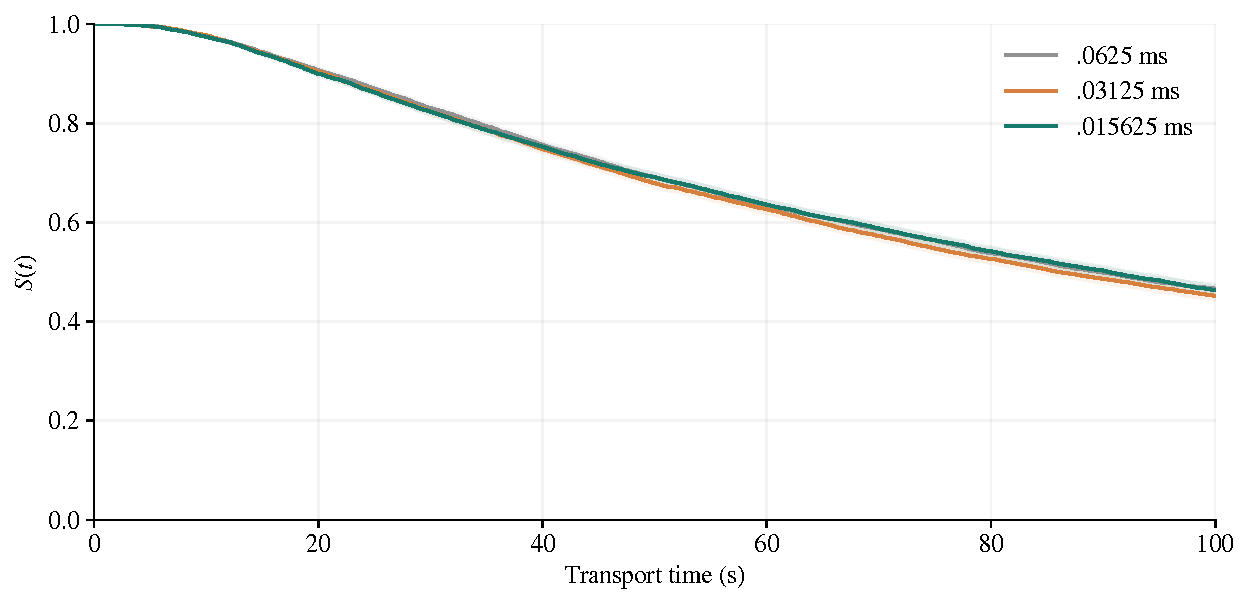
\includegraphics[width=.95\textwidth]{s4_final_survival.pdf}
\caption{Continuous-geometry survival at the three latest steps. Shading gives pointwise Wilson 95\% intervals. All curves use the same frozen local geometry, initial-center cohort, and physical diffusion coefficient.}
\end{figure}
\begin{figure}[!htbp]
\centering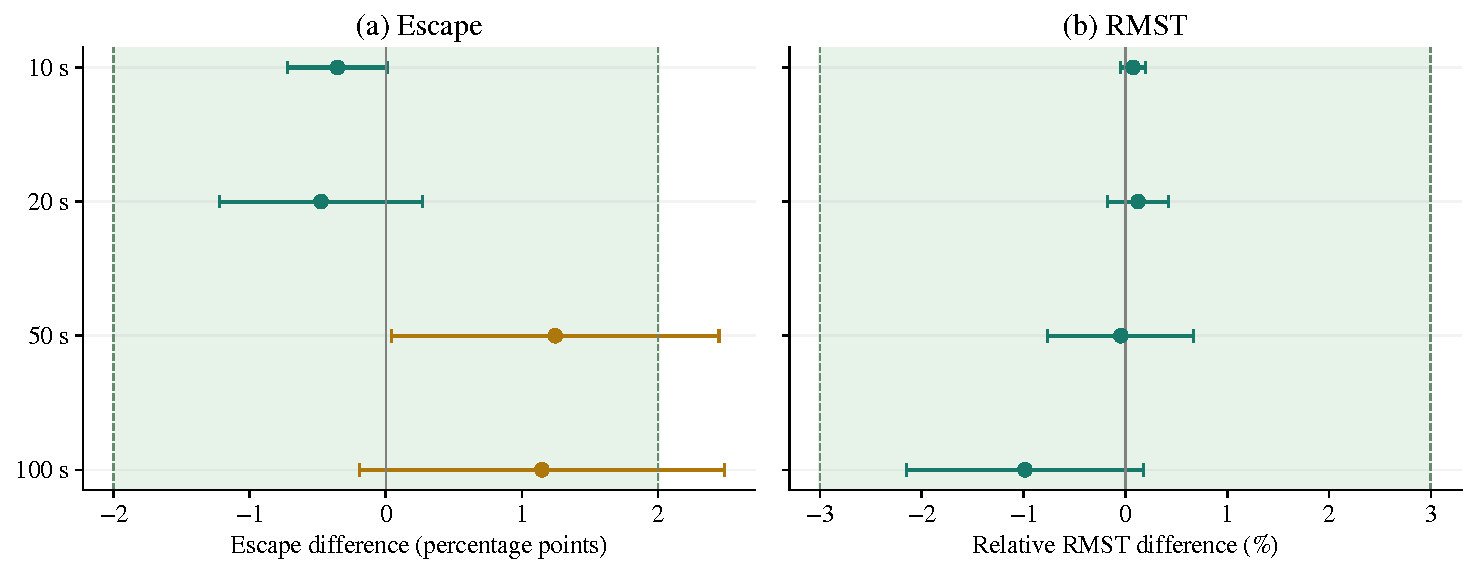
\includegraphics[width=\textwidth]{s5_final_equivalence.pdf}
\caption{Final paired temporal comparison. At 10 and 20 s both indicators meet their margins. At 50 and 100 s RMST meets its margin, but escape remains inconclusive. Green denotes within-margin intervals and amber denotes inconclusive intervals.}
\end{figure}
At 100 s the final escape interval is $[-0.194,2.489]$ pp and the relative RMST interval is $[-2.154,0.180]\%$. The phase therefore closes with RMST equivalence and unresolved joint equivalence, not a complete temporal-convergence claim. The earlier 0.0625/0.03125 ms comparison also remains inconclusive for escape.

All 32 batches were completed without outcome-dependent stopping or sample expansion. The final run took 147.32 min with four CPU processes. Its completion audit checked all 8192 new histories and reused records, source/data hashes, timing, censoring, counters, coordinate bounds, and exact empirical-survival integration. The 342 protected files were unchanged \emph{during that experiment}; subsequent authorized manuscript edits are separate from those archived audit snapshots.

\clearpage
\section{Closure and reproducibility of the historical verification}
\textbf{Supported conclusions.} The specified collision and censoring rules pass their implementation checks. The fixed $H=70$ nm mask has a practically equivalent selected time-step pair. Local conservative geometric metrics meet their per-axis criteria. The final $H=100$ nm continuous comparison meets the restricted-mean tolerance for the tested large tracer and all four horizons.

\textbf{Unresolved items.} Joint escape/RMST equivalence at 50--100 s, uniform survival-curve equivalence, the mixed-boundary analytical tolerance, full cell-versus-continuous kinetic equivalence, complete-clot boundary handling, and transport with moving obstacles are not established. Neither $H=100$ nm nor the local ROI geometry is experimentally validated here.

\textbf{Operational choice.} Preserve the continuous detector and the finest tested 0.015625 ms calculation as a reference for this specific local problem. This is not an automatic change to production defaults or validation of the reflection protocol below. A larger or evolving system requires a documented treatment of its own boundaries and geometry. No new validation run was launched for this manuscript update.

\subsection*{Data inventory}
The companion directory \path{data/validation/} contains the source CSVs used to construct the tables and figures:
\begin{itemize}
\item \path{h70_comparison.csv}, \path{h70_summary.csv}, and \path{h70_additional_batches.csv}: combined fixed-mask results and batch sensitivity.
\item \path{obstacle_controls.csv} and \path{continuous_controls.csv}: analytical benchmark comparisons.
\item \path{spatial_geometry.csv} and \path{spatial_comparisons.csv}: conservative geometry and per-axis criteria.
\item \path{cell_continuous_comparisons.csv}: new-only precision comparison across geometry and time-step methods.
\item \path{continuous_dt31_comparisons.csv}: first nested refinement.
\item \path{continuous_final_comparisons.csv}, \path{continuous_final_summary.csv}, and \path{continuous_final_survival.csv}: final refinement, censoring, and survival curves.
\end{itemize}
\path{provenance.json} records each original source path and SHA-256 hash. Figure files are in \path{figures/validation/}. Underlying per-tracer histories, seeds, configurations, source files, and completion audits remain in their original experiment directories; these were not rerun or overwritten.

The $H=70$ nm study uses batch seeds 77000--77015. The $H=100$ nm precision cohort and both nested refinements use seeds 80600--80631, with particle identity preserved within each 256-history batch. Saved final coordinates are the last accepted interior positions, not exact face-intersection coordinates. Full intermediate tracer positions are not stored, although the fixed seeds and source versions reproduce proposals.

Mechanical replicas and Monte Carlo batches are distinct sampling units. More tracers improve precision conditional on a fixed network but do not estimate uncertainty across clots. Differences between two size/diffusion scenarios are not exclusively steric, and finite-time survival alone cannot establish binding, irreversible capture, permeability, or an independent aggregation rate.

\clearpage
\section{Current full-common-domain reflection and homogeneous pilot}
\label{sec:current-reflection}
\subsection*{Distinct protocol and implementation checks}
The main-text cohort uses 50 layers with $H=100$ nm, a $0.25~\mu$m-radius tracer, $D=0.4~\mu$m$^2$/s, and continuous extrusions of backbone segments, cohesive links, and platelet disks. The lateral region is the intersection of the layer interiors on their native raster, not the central ROI of S1--S7. Its boundary reflects tracer centers directly. Both $z=0$ and $z=5~\mu$m absorb the center. Central proposals have radius $1.19~\mu$m and $z\in[2,3]~\mu$m and are accepted by clearance, without connectivity conditioning.

The remaining Gaussian displacement is geometrically reflected at the first contact. Multiple active normals are orthogonalized; their normal subspace is reflected. A contact tied with an axial exit is processed first. If 256 contacts exhaust a local budget, the same increment is subdivided geometrically, retaining noise and physical duration. This resolves a verified 713-bounce narrow-gap path; it is not Brownian time-step refinement. Numerical failures terminate a run rather than produce censored particles. The method is not the force-dependent propagator of Behringer and Eichhorn \cite{BehringerEichhorn2012}.

The reflection implementation passed 26510 test cases: 1500 analytic sphere contacts, 1500 cylinder contacts, 500 extruded-capsule checks against independent minimization, 20000 planar-image checks, 2000 lateral segment--box comparisons, 1000 multihit reversibility cases, and ten boundary-ordering, corner, and subdivision controls. These counts describe tests, not independent mechanical samples. A 4096-tracer straight-channel benchmark reduced the relative point error in RMST from 5.28\% at 0.5 ms to 1.17\% at 0.015625 ms, relative to the truncated analytical reference. It does not establish uniform error bounds over curved clot geometries.

\subsection*{Initial long-horizon temporal comparison}
On replica 1, $f_0=2.2$ nN, mechanical time 10 s, 256 paired histories compare 0.03125 and 0.015625 ms until 100 s. At the coarse step, 197 escape and 59 are censored, with RMST 58.8524 s. At the fine step, 192 escape and 64 are censored, with RMST 59.0619 s. There are 59 discordant escape pairs. Table~\ref{tab:reflection-equivalence} preserves the inconclusive decisions.

\begin{table}[htbp]
\centering\small
\caption{Initial 256-history reflection comparison, coarse minus fine. Marginal 97.5\% intervals use a Bonferroni allocation for nominal joint 95\% coverage of the two endpoints; bootstrap coverage is approximate. Original margins and decisions are preserved.}\label{tab:reflection-equivalence}
\begin{tabular}{@{}lccc@{}}
\toprule
Observable & Difference [interval] & Margin & Decision \\ \midrule
$S(100)$ & $-1.953\ [-12.238,8.408]$ pp & $\pm2$ pp & Inconclusive \\
Relative RMST & $-0.355\ [-6.865,6.650]\%$ & $\pm3\%$ & Inconclusive \\
\bottomrule
\end{tabular}
\end{table}
The survival interval uses conservative exact binomial bounds for paired discordance; RMST uses 20000 paired bootstrap resamples. Extending the horizon exposes late exits but does not increase the number of independent trajectories or establish equivalence. This initial comparison motivated the larger-sample study below. Spatial convergence of this complete-domain transport problem was not tested by either temporal comparison.

\subsection*{Larger-sample refinement and revised operational criterion}
A fixed-allocation study uses 8192 paired histories in each of three frozen states: A, replica 1 at 0 s; B, replica 1 at $f_0=2.2$ nN and 10 s; and C, replica 9 at $f_0=8.8$ nN and 15 s. These states represent two mechanical seed groups, not three independent mechanical replicas. Each state is tested at 0.03125, 0.015625, and 0.0078125 ms with a 100 s horizon, totaling 73728 verification trajectories, separate from the main-text cohort. The geometries, initial release law, reflection rules, tracer radius, and diffusivity are unchanged. New initial-position and Brownian seeds are used; within each state, all steps share the same accepted starting positions and nested Gaussian increments. No mechanical evolution was repeated.

The primary contrast is 0.015625 minus 0.0078125 ms. Survival intervals retain the same conservative construction from exact binomial bounds on positive and negative discordances. Relative RMST intervals use 20000 paired percentile-bootstrap resamples, with the finer RMST as denominator. Marginal coverage is 97.5\%, with nominal joint 95\% coverage for the two endpoints within a comparison; bootstrap coverage is approximate. Simultaneous interval coverage across all states is not claimed. The allocation and original margins, $\pm2$ pp and $\pm3\%$, were fixed before the new outcomes were inspected; no interim scientific analysis or outcome-dependent sample enlargement occurred.

\begin{table}[htbp]
\centering\small
\caption{Independent larger-sample temporal comparison: 0.015625 minus 0.0078125 ms, with 8192 paired histories per state and 100 s observation. Intervals are marginal 97.5\% intervals. Decisions use the revised survival margin of $\pm2.5$ pp and unchanged RMST margin of $\pm3\%$. The survival margin was revised after examining the results; under the original $\pm2$ pp margin, state B remains inconclusive.}
\label{tab:temporal-revised}
\begin{tabular}{@{}lccc@{}}
\toprule
State & $\Delta S$ [interval], pp & Relative RMST [interval], \% & Revised decision\\
\midrule
A: R1, $t_m=0$ s & $0.024\ [-1.398,1.447]$ & $0.338\ [-0.629,1.317]$ & Within margins\\
\specialrule{0.2pt}{1.5pt}{1.5pt}
B: R1, 2.2 nN, 10 s & $0.806\ [-0.782,2.392]$ & $0.318\ [-0.682,1.339]$ & Within margins\\
\specialrule{0.2pt}{1.5pt}{1.5pt}
C: R9, 8.8 nN, 15 s & $-0.049\ [-1.424,1.326]$ & $0.149\ [-1.067,1.385]$ & Within margins\\
\bottomrule
\end{tabular}
\end{table}


After reviewing the completed results, the operational survival tolerance was revised to $\pm2.5$ pp, retaining $\pm3\%$ for relative RMST. Under this revised criterion, both indicators meet their margins in all three states (Table~\ref{tab:temporal-revised}). Under the original survival margin, state B remains inconclusive because its interval reaches $2.392$ pp. The revised acceptance is therefore a post-analysis tolerance assessment, not confirmation of the original criterion or a biologically calibrated error threshold \cite{Lakens2017}. The intervals and raw outcomes are unchanged. At a survival level of 25\%, 2.5 pp corresponds to a 10\% relative difference, illustrating why the absolute tolerance must remain explicit.

The secondary 0.03125-minus-0.015625 ms contrasts meet even the original margins in all three states. This does not imply exact convergence or monotonic sample differences with refinement. All 1152 blocks finished without numerical failure. A legacy-noise build reproduced eight historical trajectories exactly in every recorded field; 4096 free-space paths per level verified nested increments, with maximum endpoint disagreement below $2.8\times10^{-11}~\mu$m. The selected 0.015625 ms step is retained under the revised practical criterion. This conclusion is restricted to the tested states and parameters and does not certify all 117 production geometries, uniform equivalence of $S(t)$, moving obstacles, or a revised stereological construction. Original and revised result summaries and the original protocol are retained separately in \path{data/temporal_confirmation_20261009/}.

\subsection*{Independent connectivity certification}
An auxiliary $512\times512\times100$ grid has $h_{xy}=92.96875$ nm and $h_z=50$ nm. For center-to-solid distance $d_c$ and cell half-diagonal $q$, the 1-Lipschitz distance bound gives
\begin{equation}
d_c-q\ge a+\epsilon\quad\hbox{(entirely valid)},\qquad
d_c+q\ge a-\epsilon\quad\hbox{(possibly valid)},
\end{equation}
where $\epsilon=10^{-12}~\mu$m. The inner graph uses six face neighbors, and the outer possible graph uses 26 neighbors to avoid ruling out corner-connected candidates. Both are clipped to the same common lateral region. Interior paths touching a $z$ face certify an exit connection. Up to 32 nearby exit-connected inner-cell centers within $0.5~\mu$m are also tried as endpoints of exact straight clearance-tested bridges. Failure of this bounded search is unresolved, not disconnection. Disconnection would require absence of a path even in the outer graph.

Among the 29952 unique histories, 20052 starts are independently connected, six disconnected, and 9894 unresolved. Replica 4 at 10 s has one disconnected start at 4.4 nN and two at 8.8 nN, with all remaining starts unresolved; the corresponding bounds are $[0,255/256]$ and $[0,254/256]$. At 15 s, replica 4 has one disconnected start at 2.2 nN and two at 4.4 nN. All six disconnected state-specific starts remain censored at 100 s. They involve two distinct physical coordinates reused across geometries, not six distinct pores. This is a small non-vacuous consistency check, not a general validation. The upper connectivity bound remains 100\% in states without a certified disconnected start. Replica 1 at 10 s and 4.4 or 8.8 nN has a lower bound of zero with all 256 starts unresolved, despite observed exits. Of the 6100 censored histories, 3380 start at certified connected centers, six at disconnected centers, and 2714 at unresolved centers. Geometry-classification files are preserved before the escape outcomes are used.

\subsection*{Homogeneous analysis, pairing, and provenance}
The cohort contains nine paired mechanical seed groups, four baselines, and frozen states at 0, 5, 10, and 15 s. Shared initial states reduce 144 labels to 117 geometries. The allocation is fixed at 256 histories per unique geometry. The completed six-block data at 0, 5, and 10 s supply 13824 histories unchanged, including the 256 compatible histories reused in the initial two-block pilot. Blocks 7--9 at those times add 6912 histories, and all nine blocks at 15 s add 9216, giving 29952 without double-counting shared initial states. Blocks 3--9 use consecutive groups of 50 layer seeds from 4100--4149 through 4400--4449. There are 36 force-specific stacks and 1800 layer evolutions, but only nine paired seed groups for between-replica comparisons.

The mechanical evolutions continue from their saved 10 s states to 15 s, preserving existing cohesive topology, link reference lengths, and stochastic continuation state. Original 0 s areas remain the contraction reference. The allocation was fixed before analyzing each batch, rather than all nine blocks being declared before the first pilot. Original batch protocols and execution records are retained separately. Exactly two fine-step histories contact the lateral wall: replica 8 at 2.2 nN and 10 s has one history with 981 contacts, and replica 8 at 8.8 nN and 15 s has one with 73 contacts. Thus there are 1054 lateral events in two histories, not 1054 independent particles. Neither occurs in the retained six-block subset. At the coarse step of the separate refinement comparison, one tracer also contacts the lateral wall.

Within each mechanical replica, Gaussian seeds are paired by particle index, but geometry-conditioned accepted initial positions can differ. Main-text contrast intervals use 10000 paired-index percentile bootstrap resamples \cite{Efron1979}, with analysis seed 20260919 and replica draw order 1--9. This retains the original draws, metrics, and contrast intervals for replicas 1--6 at 0, 5, and 10 s. The same replica-specific index matrix is also used for 15-minus-10 s comparisons. Intervals quantify approximate conditional tracer-sampling variation, not between-network uncertainty, all initial-proposal dependence, or numerical bias. They are marginal rather than simultaneous. Supplementary CSVs retain both same-index initial matches and common physical positions independent of index. Force-control pairs share 26--225 physical coordinates among 256 starts, with at most 68 also matched by index.

The directory \path{data/homogeneous_pilot/} contains state metrics, geometry metrics, paired contrasts, survival horizons, connectivity counts, merged event histories, and per-start connectivity/escape classifications. Its provenance file records source paths and SHA256 hashes. The geometry and transport sources remain distinct from \path{data/validation/}, which stores the historical studies. No obsolete endpoint, rejection-only, or cohesion-omitting trajectories enter the homogeneous tables.

\textbf{Scope at closure.} The present result is a reproducible, frozen-state descriptive pilot. Nine mechanical replicas expose between-realization heterogeneity but do not establish population robustness; unresolved connectivity is not physical isolation; and no external structural or mechanical validation has been completed. The selected time step meets revised practical tolerances in three tested states, including one at 15 s; the original survival tolerance remains inconclusive in one state. Complete temporal/spatial convergence over the production cohort is not claimed. Further replicas, stronger connectivity certificates, and moving-network transport remain proposed continuations.

\bibliographystyle{unsrt}
\begingroup
\small
\setlength{\parskip}{0pt}
\bibliography{refs}
\endgroup
\end{document}
